% Shared content for Mock Exam 1. Driven by Mock-Exam-1-Questions.tex
% (\solutionsfalse) and Mock-Exam-1-Solutions.tex (\solutionstrue).
\documentclass[11pt]{article}
\usepackage[a4paper,margin=2.2cm]{geometry}
\usepackage{graphicx}
\usepackage{amsmath}
\usepackage{xcolor}
\usepackage{enumitem}
\usepackage{fancyhdr}
\usepackage{tikz}
\usetikzlibrary{shapes,arrows.meta,positioning,calc}
\usepackage{caption}

\graphicspath{{figures/}}
\definecolor{ansgreen}{RGB}{0,130,40}
\definecolor{trapred}{RGB}{180,30,30}

\pagestyle{fancy}
\fancyhf{}
\rhead{\small 16 questions LC1 mock exam 31.05.2026}
\cfoot{\small Page \thepage}
\renewcommand{\headrulewidth}{0pt}

\setlist[enumerate,2]{label=\arabic*., leftmargin=1.6em, itemsep=2pt, topsep=3pt}

% Worked-answer block: only rendered in the Solutions build.
\newcommand{\solution}[1]{%
  \ifsolutions
    \par\smallskip
    \noindent\fcolorbox{ansgreen}{ansgreen!6}{%
      \parbox{\dimexpr\linewidth-2\fboxsep-2\fboxrule}{%
        \small\textbf{\color{ansgreen}Answer.} #1}}%
    \par\medskip
  \fi}

% A 2x2 grid of option figures, each captioned with its option number.
\newcommand{\optfig}[2]{%
  \parbox[t]{0.46\linewidth}{\centering
    \textbf{#2.}\\[2pt]\includegraphics[width=\linewidth]{#1}}}

\newcommand{\qhead}[1]{\bigskip\noindent\textbf{#1}\par\nobreak\smallskip}

\title{\vspace{-1.5cm}\Huge EXAM Linear Control Design 1\\[4pt]
  \large 31 May 2026 --- Questions, Multiple Choice\\[-4pt]}
\date{}
\author{}

\begin{document}
\maketitle
\thispagestyle{fancy}
\vspace{-1.4cm}
\noindent\rule{\linewidth}{0.4pt}\par
\ifsolutions
  \begin{center}\large\textbf{\color{ansgreen}SOLUTIONS --- with worked reasoning}\end{center}
\else
  \begin{center}\small Each question is worth \textbf{(1 Point)}. Choose the single best answer.
  You may use the LCD1 Exam Suite app.\end{center}
\fi
\medskip

%==================================================================== Q1
\qhead{Q1. Consider the block diagram in Fig.~1. What is the closed-loop
transfer function $\dfrac{Y(s)}{R(s)}$? (1 Point)}

\begin{center}
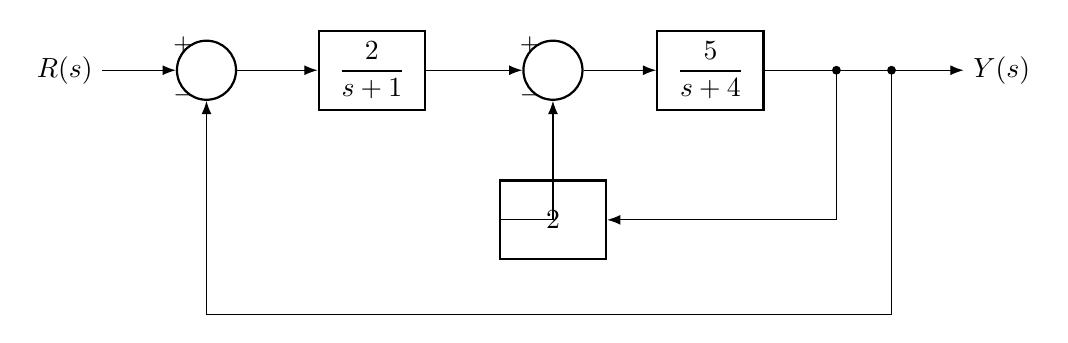
\begin{tikzpicture}[>=Latex,
   block/.style={draw,thick,rectangle,minimum height=1.0cm,minimum width=1.35cm},
   sum/.style={draw,thick,circle,minimum size=7.5mm,inner sep=0pt}]
 % forward-path nodes (explicit coordinates for a clean layout)
 \node (in)  at (0,0)    {$R(s)$};
 \node[sum]   (s1) at (1.8,0)  {};
 \node[block] (g1) at (3.9,0)  {$\dfrac{2}{s+1}$};
 \node[sum]   (s2) at (6.2,0)  {};
 \node[block] (g2) at (8.2,0)  {$\dfrac{5}{s+4}$};
 \coordinate (p) at (9.8,0);    % inner take-off
 \coordinate (q) at (10.5,0);   % outer take-off
 \node (out) at (11.9,0) {$Y(s)$};
 \node[block] (h2) at (6.2,-1.9) {$2$};
 % forward wires
 \draw[->] (in) -- (s1);
 \draw[->] (s1) -- (g1);
 \draw[->] (g1) -- (s2);
 \draw[->] (s2) -- (g2);
 \draw (g2) -- (q);
 \draw[->] (q) -- (out);
 \fill (p) circle (1.6pt);
 \fill (q) circle (1.6pt);
 % summing-junction signs (at the entering ports)
 \node[font=\small] at ($(s1.north west)+(-0.02,0.04)$) {$+$};
 \node[font=\small] at ($(s1.south west)+(-0.02,-0.04)$) {$-$};
 \node[font=\small] at ($(s2.north west)+(-0.02,0.04)$) {$+$};
 \node[font=\small] at ($(s2.south west)+(-0.02,-0.04)$) {$-$};
 % inner feedback H2 = 2  (p -> down -> H2 -> up into s2 from below)
 \draw[->] (p) |- (h2.east);
 \draw[->] (h2.west) -| (s2.south);
 % outer unity feedback  (q -> down -> left -> up into s1 from below)
 \draw[->] (q) -- ++(0,-3.1) -| (s1.south);
\end{tikzpicture}\\[3pt]
{\small Figure 1: Block diagram ($H_2=2$, outer unity feedback).}
\end{center}

\begin{enumerate}
\item[]\begin{enumerate}
 \item $\dfrac{10}{s^{2}+15s+24}$
 \item $\dfrac{10}{s^{2}+15s+14}$
 \item $\dfrac{10}{s^{2}+5s+24}$
 \item $\dfrac{5}{s^{2}+15s+24}$
\end{enumerate}\end{enumerate}
\solution{Reduce the inner loop first: $\dfrac{5/(s+4)}{1+2\cdot 5/(s+4)}
=\dfrac{5}{s+14}$. In series with $G_1$: $\dfrac{2}{s+1}\cdot\dfrac{5}{s+14}
=\dfrac{10}{(s+1)(s+14)}$. Closing the unity loop:
$\dfrac{10}{(s+1)(s+14)+10}=\dfrac{10}{s^{2}+15s+24}$. \textbf{Option 1.}
\emph{App:} Block Diagram mode --- draw the three blocks + two feedbacks, read off
$G(s)$. CLI cross-check: \texttt{tf "10/(s**2+15*s+24)"}.}

%==================================================================== Q2
\qhead{Q2. A system is described by the differential equation
$\ddot{y}+4\dot{y}+13y=2u$. What are the poles of its transfer function? (1 Point)}
\begin{enumerate}\item[]\begin{enumerate}
 \item $s=-2\pm 3j$
 \item $s=-2\pm 3.6j$
 \item $s=-0.5\pm 1.8j$
 \item $s=-4\pm 13j$
\end{enumerate}\end{enumerate}
\solution{Characteristic polynomial $s^{2}+4s+13=0\Rightarrow
s=-2\pm\sqrt{4-13}=-2\pm 3j$. \textbf{Option 1.} (Distractor 2 uses
$\omega_n=\sqrt{13}=3.6$ instead of the damped frequency.)
\emph{App:} \texttt{ode --y "1,4,13" --u "2"} $\to$ $-2\pm 3j$.}

%==================================================================== Q3
\qhead{Q3. A system has the state-space model
$A=\begin{bmatrix}-2&1\\0&-3\end{bmatrix}$,
$B=\begin{bmatrix}0\\1\end{bmatrix}$,
$C=\begin{bmatrix}1&0\end{bmatrix}$, $D=0$.
What is the transfer function $G(s)=Y(s)/U(s)$? (1 Point)}
\begin{enumerate}\item[]\begin{enumerate}
 \item $\dfrac{1}{s^{2}+5s+6}$
 \item $\dfrac{1}{s^{2}+5s+5}$
 \item $\dfrac{s}{s^{2}+5s+6}$
 \item $\dfrac{1}{s^{2}+6s+6}$
\end{enumerate}\end{enumerate}
\solution{$G(s)=C(sI-A)^{-1}B=\dfrac{1}{(s+2)(s+3)}=\dfrac{1}{s^{2}+5s+6}$,
poles $-2,-3$, DC gain $1/6\approx0.167$. \textbf{Option 1.}
\emph{App:} \texttt{ss --A "[[-2,1],[0,-3]]" --B "[[0],[1]]" --C "[[1,0]]"}.}

%==================================================================== Q4
\qhead{Q4. Consider the second-order system
$G(s)=\dfrac{25}{s^{2}+3s+25}$.
Which plot is its unit step response? (1 Point)}
\begin{center}
\optfig{q4_step_a.png}{1}\hfill\optfig{q4_step_b.png}{2}\\[6pt]
\optfig{q4_step_c.png}{3}\hfill\optfig{q4_step_d.png}{4}
\end{center}
\solution{$\omega_n=\sqrt{25}=5$, $2\zeta\omega_n=3\Rightarrow\zeta=0.30$
(under-damped). Overshoot $M_p=e^{-\pi\zeta/\sqrt{1-\zeta^2}}\approx 37\%$,
$t_p=\pi/\omega_d=\pi/(5\sqrt{1-0.09})\approx0.66$\,s.
\textbf{Option 1} (Plot~2 is $\zeta=0.7$, Plot~3 $\zeta=0$, Plot~4 over-damped).
\emph{App gap:} pick-the-plot is \emph{not} solver-shaped. The student can confirm
the shape with \texttt{characterize "25/(s**2+3*s+25)"} ($M_p\approx0.37$, $\zeta=0.3$)
and match it to Plot~1.}

%==================================================================== Q5
\qhead{Q5. For $G(s)=\dfrac{20}{(s+2)(s+5)}$, what is the DC gain expressed
\emph{in decibels}? (1 Point)}
\begin{enumerate}\item[]\begin{enumerate}
 \item $6.0$ dB
 \item $2.0$ dB
 \item $26$ dB
 \item $-6.0$ dB
\end{enumerate}\end{enumerate}
\solution{$G(0)=\dfrac{20}{2\cdot5}=2$ (linear). In dB:
$20\log_{10}2=6.0$ dB. \textbf{Option 1.}
\emph{Trap:} Option~2 is the \emph{linear} value $2$ mislabelled as ``dB'';
Option~3 takes $20\log_{10}20$ and forgets the poles.
\emph{App:} \texttt{tf "20/((s+2)*(s+5))"} prints ``DC gain 2 (6.02 dB)'' --- both
forms, so the unit is unambiguous.}

%==================================================================== Q6
\qhead{Q6. The Bode plot of an open-loop transfer function $G(s)$ is shown in
Fig.~2. Determine $G(s)$. (1 Point)}
\begin{center}
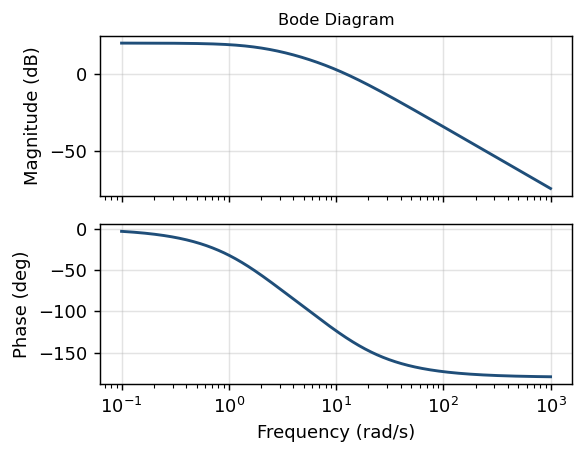
\includegraphics[width=0.62\linewidth]{q6_bode.png}\\[3pt]
{\small Figure 2: Bode diagram of $G(s)$.}
\end{center}
\begin{enumerate}\item[]\begin{enumerate}
 \item $\dfrac{200}{(s+2)(s+10)}$
 \item $\dfrac{10}{(s+2)(s+10)}$
 \item $\dfrac{200}{(s+1)(s+5)}$
 \item $\dfrac{100}{(s+2)(s+10)}$
\end{enumerate}\end{enumerate}
\solution{Low-frequency magnitude $\approx 20$ dB $\Rightarrow$ DC gain $=10$.
Corner frequencies (slope breaks of $-20$ dB/dec) at $\omega=2$ and $\omega=10$
$\Rightarrow$ poles at $-2,-10$. So
$G(s)=\dfrac{10}{(1+s/2)(1+s/10)}=\dfrac{200}{(s+2)(s+10)}$. \textbf{Option 1}
(Option~2 has DC gain $0.5=-6$ dB). \emph{App:}
\texttt{bode --dc 20 --corners "2:-20,10:-20" --phase "2:-90,10:-90"}
$\to$ gain 200, poles $-2,-10$.}

%==================================================================== Q7
\qhead{Q7. An open-loop transfer function has a \emph{pole at the origin}, one
\emph{real zero at $-10$}, and a pair of \emph{lightly damped complex poles}
($\omega_n=30$, $\zeta\approx0.1$). Which Bode plot corresponds to it? (1 Point)}
\begin{center}
\optfig{q7_bode_a.png}{1}\hfill\optfig{q7_bode_b.png}{2}\\[6pt]
\optfig{q7_bode_c.png}{3}\hfill\optfig{q7_bode_d.png}{4}
\end{center}
\solution{The integrator gives a $-20$ dB/dec slope and $-90^\circ$ at low
frequency; the real zero adds $+20$ dB/dec and $+90^\circ$ near $\omega=10$; the
lightly damped poles give a sharp resonance peak and a $-180^\circ$ dive near
$\omega=30$. Only \textbf{Plot~1} shows all three. (Plot~2 has no integrator,
Plot~3 a RHP zero, Plot~4 heavily damped poles with no peak.)
\emph{App gap:} pick-the-plot --- reason it out, the solver cannot eyeball figures.}

%==================================================================== Q8
\qhead{Q8. For the loop transfer function $L(s)=\dfrac{5}{s(s+1)(s+3)}$,
find the gain margin (GM) and phase margin (PM). (1 Point)}
\begin{enumerate}\item[]\begin{enumerate}
 \item GM $\approx 7.6$ dB, \quad PM $\approx 23^\circ$
 \item GM $\approx 2.4$ dB, \quad PM $\approx 23^\circ$
 \item GM $\approx 7.6$ dB, \quad PM $\approx 45^\circ$
 \item GM $\approx 15.6$ dB, \quad PM $\approx 60^\circ$
\end{enumerate}\end{enumerate}
\solution{Phase crossover at $\omega_{pc}=\sqrt{3}=1.73$ where
$|L|=5/(\omega_{pc}\cdot\sqrt{\omega_{pc}^2+1}\cdot\sqrt{\omega_{pc}^2+9})$ gives
GM $=2.4$ (linear) $=7.6$ dB; gain crossover at $\omega_{gc}=1.07$ gives
PM $=23.4^\circ$. \textbf{Option 1.} \emph{Trap:} Option~2 quotes the
\emph{linear} GM $2.4$ as if it were dB. \emph{App:}
\texttt{margins "5/(s*(s+1)*(s+3))"}.}

%==================================================================== Q9
\qhead{Q9. The plant $G(s)=\dfrac{K}{(s+1)(s+2)(s+4)}$ is placed in a unity
feedback loop. For what range of $K$ is the closed loop stable? (1 Point)}
\begin{enumerate}\item[]\begin{enumerate}
 \item $0<K<90$
 \item $0<K<14$
 \item $0<K<98$
 \item $K>0$ (stable for all positive $K$)
\end{enumerate}\end{enumerate}
\solution{Characteristic polynomial $s^{3}+7s^{2}+14s+(8+K)$. Routh first
column requires $\dfrac{7\cdot14-(8+K)}{7}>0\Rightarrow K<90$ and $8+K>0$.
So $0<K<90$. \textbf{Option 1.} \emph{App:}
\texttt{stable-k "1/((s+1)*(s+2)*(s+4))"} $\to$ $(0,90)$.}

%==================================================================== Q10
\qhead{Q10. Which Nyquist plot corresponds to
$L(s)=\dfrac{10}{s(s+1)(s+2)}$? (1 Point)}
\begin{center}
\optfig{q10_nyquist_a.png}{1}\hfill\optfig{q10_nyquist_b.png}{2}\\[6pt]
\optfig{q10_nyquist_c.png}{3}\hfill\optfig{q10_nyquist_d.png}{4}
\end{center}
\solution{$L$ has one integrator (type 1) so $|L|\to\infty$ as
$\omega\to0$ --- the curve comes \emph{from infinity}, ruling out the
finite-start Plots~2 and~4 (type~0). With three poles the phase sweeps
$-90^\circ\to-270^\circ$, a single large loop without the extra upper-half
excursion of the type-2 Plot~3. \textbf{Plot~1.}
\emph{App gap:} pick-the-plot. The student may still get the encirclement count
from \texttt{stability "10/(s*(s+1)*(s+2))"} to reason about it.}

%==================================================================== Q11
\qhead{Q11. The unity-feedback system with open-loop transfer function
$G(s)=\dfrac{20}{s(s+2)(s+5)}$ is driven by a \emph{unit ramp} input.
What is the steady-state error? (1 Point)}
\begin{enumerate}\item[]\begin{enumerate}
 \item $0.5$
 \item $0$
 \item $\infty$
 \item $0.05$
\end{enumerate}\end{enumerate}
\solution{One pole at the origin $\Rightarrow$ type 1. Velocity constant
$K_v=\lim_{s\to0}sG(s)=\dfrac{20}{2\cdot5}=2$, so
$e_{ss}=1/K_v=0.5$. \textbf{Option 1.} \emph{App:}
\texttt{ess "20/(s*(s+2)*(s+5))"} $\to$ type 1, $K_v=2$, ess(ramp)$=0.5$.}

%==================================================================== Q12
\qhead{Q12. A unity-feedback system has the \emph{closed-loop} transfer
function $\dfrac{K}{s^{2}+4s+K}$. Choose $K$ so that the unit-step overshoot
is $10\%$. (1 Point)}
\begin{enumerate}\item[]\begin{enumerate}
 \item $K\approx 11.4$
 \item $K\approx 16$
 \item $K\approx 4$
 \item $K\approx 25$
\end{enumerate}\end{enumerate}
\solution{$\omega_n=\sqrt{K}$, $2\zeta\omega_n=4\Rightarrow\zeta=2/\sqrt{K}$.
$M_p=10\%\Rightarrow\zeta=0.591\Rightarrow\sqrt{K}=2/0.591=3.38\Rightarrow K=11.4$.
\textbf{Option 1.} (Option~2: $\zeta=0.5$ gives $16\%$ overshoot.)
\emph{App:} \texttt{closed-loop "K/(s**2+4*s+K)" --kind Mp --value 0.1}
$\to$ $K=11.45$, $\zeta=0.591$.
\emph{Note:} \texttt{k-for-spec} on the same string returns $10.45$ --- it treats
the argument as an \emph{open}-loop $L$ and forms $L/(1{+}L)$, a different problem.
Use the \texttt{closed-loop} form when the TF given is already the closed loop.}

%==================================================================== Q13
\qhead{Q13. A PI-Lead controller
$C(s)=K_P\big(1+\tfrac{1}{\tau_i s}\big)\dfrac{1+\tau_d s}{1+\alpha\tau_d s}$
is designed for the plant
$G(s)=\dfrac{900}{(0.25s+1)(s^{2}+50s+3000)}$, with lead ratio
$\alpha=0.01$ and integral corner $1/\tau_i=\omega_c/3$. Find $K_P$ that
places the gain crossover at $\omega_c$ with phase margin $75^\circ$. (1 Point)}
\begin{enumerate}\item[]\begin{enumerate}
 \item $K_P\approx 3.41$
 \item $K_P\approx 0.34$
 \item $K_P\approx 34$
 \item $K_P\approx 1.0$
\end{enumerate}\end{enumerate}
\solution{The lead and PI terms set the controller phase at $\omega_c$; the
magnitude condition $|C(j\omega_c)G(j\omega_c)|=1$ then fixes $K_P=3.41$.
\textbf{Option 1.} \emph{App:}
\texttt{pi-lead --unknown KP --G "900/((0.25*s+1)*(s**2+50*s+3000))"
--gammaM 75 --alpha 0.01 --Ni 3} $\to K_P=3.414$.}

%==================================================================== Q14
\qhead{Q14. For the loop transfer function $L(s)=\dfrac{1}{s(s+21)}$,
find the proportional gain $K_P$ giving a phase margin of $45^\circ$. (1 Point)}
\begin{enumerate}\item[]\begin{enumerate}
 \item $K_P=6.24$
 \item $K_P=8.4$
 \item $K_P=0.62$
 \item $K_P=62$
\end{enumerate}\end{enumerate}
\solution{\textbf{Planted data/answer mismatch (a real exam misprint pattern).}
With the \emph{printed} plant $1/(s(s+21))$, the gain for PM $=45^\circ$ is
$K_P=623.7$ --- which matches \emph{none} of the options. The option list was
built for $1/(s(s{+}2.1))$, which gives $K_P=6.24$ (Option~1). So the printed
``$s+21$'' is a typo for ``$s+2.1$''.
\emph{App behaviour:} Smart Paste in the app computes $623.7$ and the option
matcher returns ``\,closest, but 90\% off\,'' --- it \emph{refuses to crown a
match} rather than bluffing Option~1. \emph{Finding:} the CLI
\texttt{question} command prints $623.7$ but does \emph{not} run the option
matcher, so it gives no mismatch warning --- the two Smart-Paste interfaces
disagree.}

%==================================================================== Q15
\qhead{Q15. A nonlinear system is governed by
$\ddot{x}+\dot{x}+4\sin(x)=u$. It is held at the operating point
$x_0=\pi/3$ by a constant input. Linearise about this point and give the
transfer function $\dfrac{\delta X(s)}{\delta U(s)}$. (1 Point)}
\begin{enumerate}\item[]\begin{enumerate}
 \item $\dfrac{1}{s^{2}+s+2}$
 \item $\dfrac{1}{s^{2}+s+4}$
 \item $\dfrac{1}{s^{2}+s+3.46}$
 \item $\dfrac{1}{s+2}$
\end{enumerate}\end{enumerate}
\solution{Linearising $4\sin(x)$ about $x_0$ gives
$4\cos(x_0)\,\delta x$. With $x_0=\pi/3$, $4\cos(\pi/3)=4(0.5)=2$, so
$\delta\ddot{x}+\delta\dot{x}+2\,\delta x=\delta u\Rightarrow
\dfrac{1}{s^{2}+s+2}$ (poles $-0.5\pm1.32j$). \textbf{Option 1.}
\emph{Traps:} Option~2 uses the coefficient $4$ (i.e.\ linearises at $x=0$);
Option~3 wrongly uses $4\sin(\pi/3)=3.46$.
\emph{App gap:} the solver \emph{cannot linearise} --- the student must do it by
hand, then may verify the result with \texttt{tf "1/(s**2+s+2)"}.}

%==================================================================== Q16
\qhead{Q16. Which of the following statements is \emph{correct}? (1 Point)}
\begin{enumerate}\item[]\begin{enumerate}
 \item Increasing the proportional gain of a unity-feedback loop generally
   raises the closed-loop bandwidth but reduces the phase margin.
 \item A lead compensator is used mainly to reduce the steady-state error.
 \item The phase margin is the extra gain (in dB) that may be added before the
   loop becomes unstable.
 \item A larger damping ratio $\zeta$ always gives a shorter rise time.
\end{enumerate}\end{enumerate}
\solution{\textbf{Option 1.} Higher gain pushes the gain-crossover frequency up
(more bandwidth, faster response) and typically eats into phase margin.
Option~2 describes a \emph{lag}/integral action; Option~3 defines the
\emph{gain} margin; Option~4 is false --- higher $\zeta$ \emph{slows} the rise.
\emph{App gap:} conceptual true/false is not solver-shaped.}

\end{document}
